\section{Einrichtung und Entwicklung des ``GReQL Converter''}\label{sec:greql-converter}

Der GReQL Converter stellt eine Webanwendung dar, die es ermöglicht, GReQL-Regeln aus einem UML-Klassendiagramm zu
extrahieren, das mithilfe von PlantText erstellt wurde. Diese extrahierten Regeln dienen anschließend der Bewertung
von UML-Klassendiagrammen auf der JACK-Plattform. Die Realisierung dieser Anwendung erfolgte mit dem Vue.js-Framework
im Frontend und Node.js im Backend, wie in fig-~\ref{fig:infrastructure} veranschaulicht. In diesem Kapitel wird der
Implementierungsprozess der Plattform sowie ihrer verschiedenen Komponenten ausführlich erläutert.

\begin{figure}[h]
    \centering
    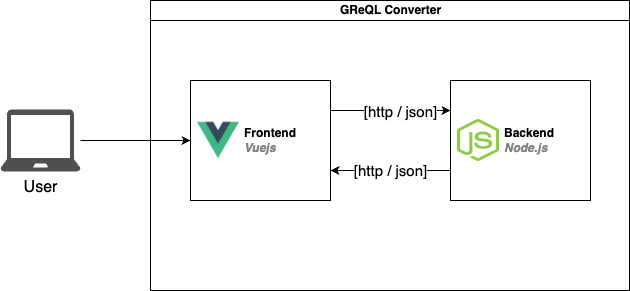
\includegraphics[width=15cm]{images/infrastucture}
    \caption{GReQL-Converter global infrastructure}
    \label{fig:infrastructure}
\end{figure}

\subsection{Einrichtung des PlantUML-Parsers}\label{subsec:einrichtung-des-plantuml-parsers}

Die Entwicklungsphase der Anwendung startete mit der Konfiguration des PlantUML-Parsers. Das ursprüngliche Ziel bestand
darin, eine Anwendung zu entwickeln, die in der Lage ist, PlantText-Code als Eingabe zu akzeptieren und als Ausgabe ein
JSON zu generieren, welches später zur Modellierung von Regelobjekten verwendet werden könnte. Ursprünglich war geplant,
den Parser direkt im Frontend einzusetzen. Es stellte sich jedoch heraus, dass der Parser nur in einer Serverumgebung
effektiv funktioniert. An dieser Stelle gab es zwei Optionen zur Auswahl: die Verwendung eines Tomcat-Servers mit Java
oder eines Node.js-Servers mit JavaScript. Die zweite Option erwies sich als die geeignetere Wahl, da sie es ermöglichte,
dieselbe Programmiersprache für das gesamte Projekt beizubehalten und die Gesamtarchitektur des Systems, einschließlich
seiner zukünftigen Bereitstellung, zu vereinfachen. Node.js eignet sich besonders gut für kleinere Projekte wie dieses.

Im Großen und Ganzen wurde Node.js ausschließlich für die Bereitstellung des Parsers genutzt, was den Backend-Code
erheblich vereinfachte~\ref{lst:bakcend}. Dies ermöglichte einen reibungslosen Übergang zum nächsten Schritt, nämlich
der Erstellung des Grunddesigns der Anwendung.

\subsection{Erstellung des Grunddesigns der Anwendung}\label{subsec:erstellung-des-grunddesigns-der-anwendung}

Um die Ziele des GReQL Converters zu erreichen, ist es von entscheidender Bedeutung, den Benutzern eine elegante,
intuitive und benutzerfreundliche grafische Benutzeroberfläche zur Verfügung zu stellen. Die möglichen Aktionen müssen
auf den ersten Blick leicht erkennbar sein, um das Verständnis zu fördern und dem Benutzer eine schnelle und effiziente
Arbeit zu ermöglichen~\cite{guntupalli2008user}. Die Seite ``Class Converter'' stellt die Benutzeroberfläche dar, auf
der der Benutzer seinen PlantText-Code in GReQL-Code umwandeln kann. Diese Seite ist in drei Hauptabschnitte unterteilt:

\begin{figure}
    \centering
    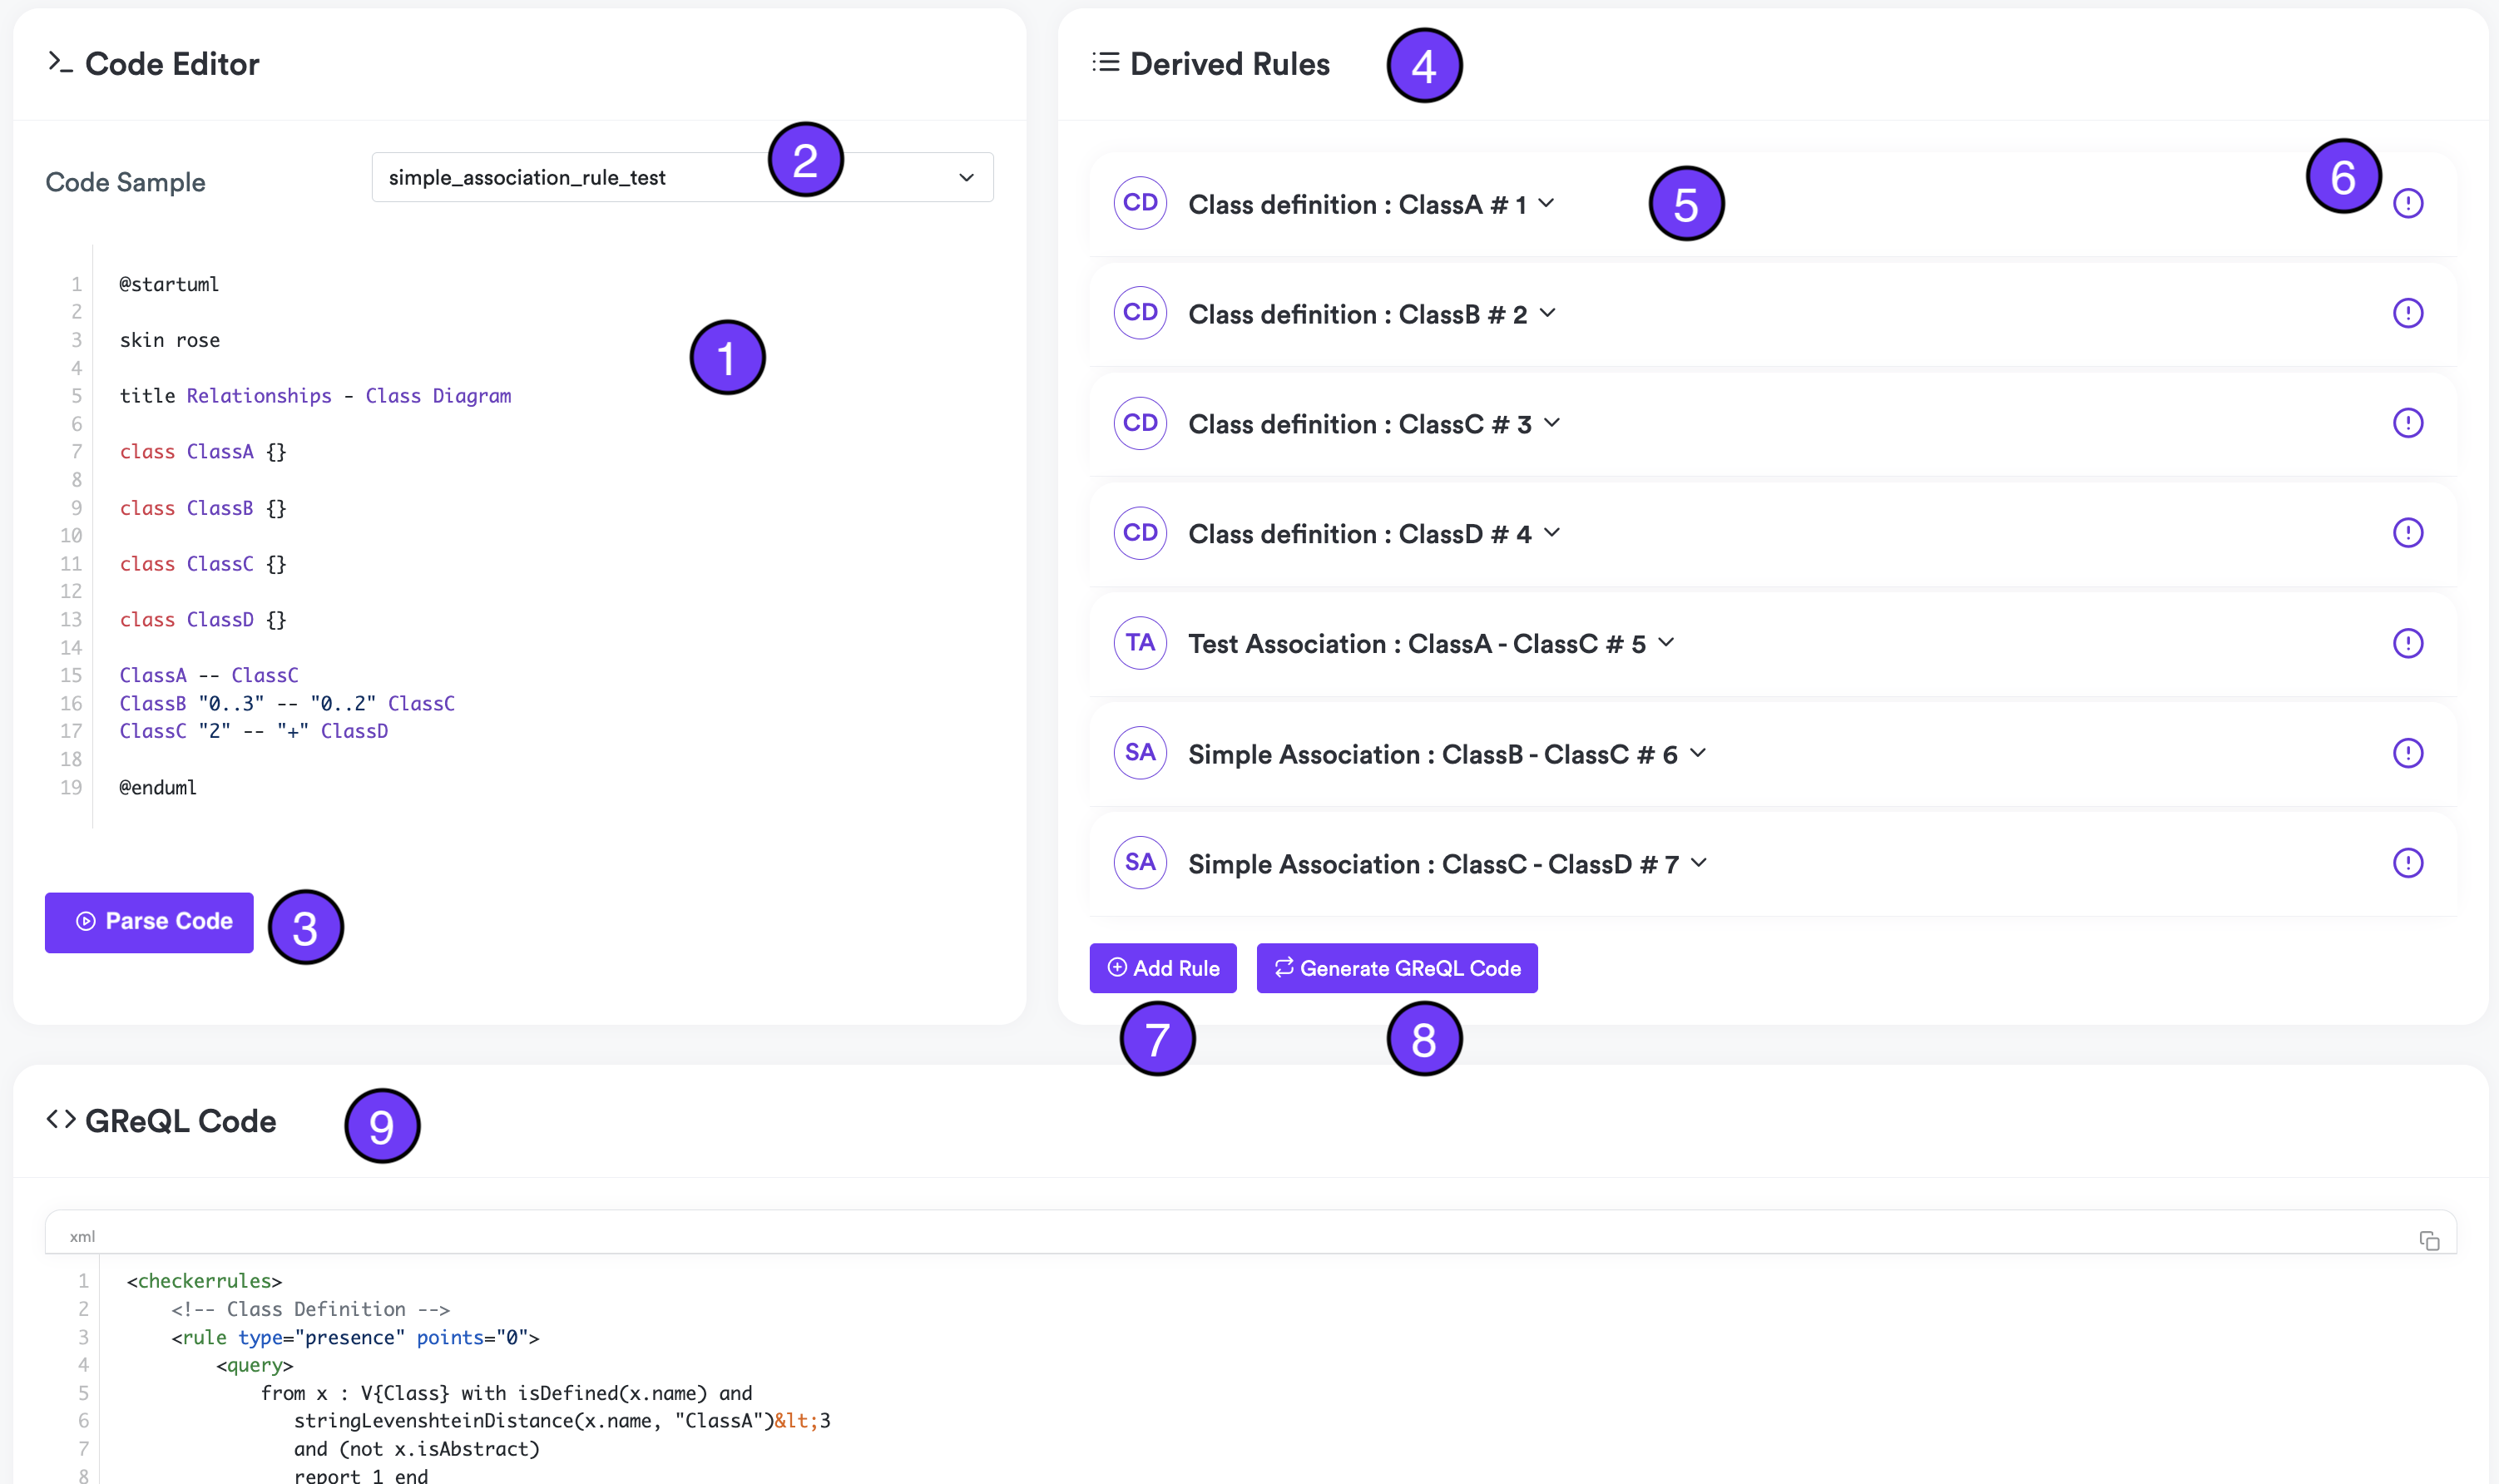
\includegraphics[width=16cm]{images/board}
    \caption{Dashboard im Überblick}
    \label{fig:dashboard}
\end{figure}

\subsubsection{Teil 1: Code editor}

Dieser Abschnitt der grafischen Benutzeroberfläche ist für die Eingabe des PlantUML-Codes durch den Benutzer vorgesehen.
Nachdem der Benutzer die Musterlösung in PlantText modelliert hat, muss er den generierten Code kopieren und in den
Editor einfügen, der durch die Nummer 1 (siehe~\ref{fig:dashboard}) gekennzeichnet ist. Darüber hinaus hat der Benutzer die
Möglichkeit, Beispielscodes auszuwählen, wie dies in PlantText der Fall ist und in der Abbildung unter Nummer 2 (siehe~\ref{fig:dashboard})
dargestellt ist. Da der geschriebene Code jedoch der in der Dokumentation definierten Struktur entsprechen muss, sind
diese Beispielscodes für den Benutzer nützlich, da sie funktionierende Codebeispiele liefern, von denen er sich
inspirieren lassen und seinen eigenen Code schreiben kann, um die Plattform zu testen. Schließlich ermöglicht der
Button ``Parse Code'' (Nummer 3 - siehe~\ref{fig:dashboard}) das Extrahieren der Regelobjekte aus dem Code, was uns zum
Teil 2 führt.

\subsubsection{Teil 2: Derived Rules}

Nachdem der Benutzer auf den Button ``Parse Code'' geklickt hat, wird eine Reihe von Regelobjekten
(Nummer 4 - siehe~\ref{fig:dashboard}) aus dem im Code-Editor vorhandenen Code generiert. Diese Regeln werden durch ein
Symbol und einen Titel dargestellt, was es ermöglicht, sie schnell zu unterscheiden und zu identifizieren. Ganz rechts
neben dem Regelobjekt befindet sich ein Ausrufezeichen, das tatsächlich ein Button ist (Nummer 6 - siehe~\ref{fig:dashboard}).
Wenn auf diesen Button geklickt wird, öffnet sich eine Dokumentation, die erklärt, was die Regel ist und wie sie
verwendet wird. Wenn der Benutzer auf die Regel klickt (Nummer 5 - siehe ~\ref{fig:dashboard}), öffnet sich ein Menü,
das es ihm ermöglicht, die in der Regel vorhandenen Informationen nach Belieben zu ändern (siehe~\ref{fig:rule_exemple}),
wodurch der GReQL Converter zu einem halbautomatischen Werkzeug wird. Diese Informationen variieren je nach Art der Regel
und den für die Generierung des GReQL-Codes erforderlichen Informationen.

\begin{figure}[h]
    \centering
    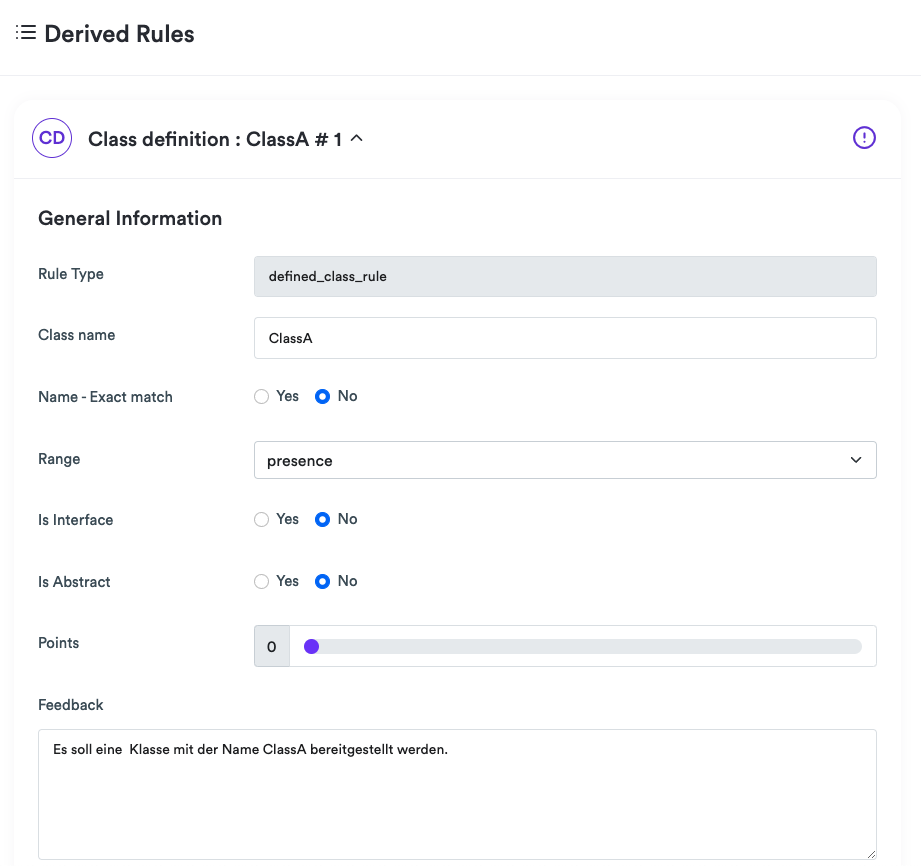
\includegraphics[width=16cm]{images/derived_rule}
    \caption{Beispiel eines Regelobjekts}
    \label{fig:rule_exemple}
\end{figure}

Dann gibt es der Button ``Add Rule'' (Nummer 7 - siehe~\ref{fig:dashboard}), die es dem Benutzer ermöglicht,
zusätzliche Regeln hinzuzufügen. Nachdem die Konfiguration und die Änderungen abgeschlossen sind, kann der Benutzer den
GReQL-Code generieren, indem er auf den Button ``Generate GReQL Code'' klickt (Nummer 8 - siehe~\ref{fig:dashboard}).
Der GReQL-Code wird aus den zuvor vom Benutzer konfigurierten Regelobjekten generiert.

\subsubsection{Teil 3: GReQL Editor}

Genau wie der erste Abschnitt ist dieser Bereich auch ein Code-Editor, jedoch für XML, da der GReQL-Code im XMI-Format
vorliegt (das auf XML basiert). Dieser Editor (Nummer 9 - siehe~\ref{fig:dashboard}) ermöglicht es erfahrenen
Benutzern, die bereits Erfahrung mit GReQL haben, detaillierte und fortgeschrittene Änderungen am generierten Code
vorzunehmen. Auf diese Weise können sie die Abfragen verbessern und spezifizieren, wenn sie sie zu allgemein finden,
oder sie einfach anpassen, je nachdem, was sie im UML-Diagramm bewerten möchten.

Diese drei verschiedenen Teile bilden das grundlegende Design des GReQL Converters. Es gibt auch andere Seiten wie die
Dokumentation oder die Startseite, die nicht erwähnt wurden, da sie in der weiteren Entwicklung keine wesentliche Rolle
spielen. Dieses Design bietet jedoch die Möglichkeit zur Erweiterung, um die Hinzufügung weiterer Seiten und sogar
weiterer Parser zu erleichtern. Der nächste Abschnitt konzentriert sich auf den Prozess der Extraktion von Regelobjekten
aus dem zuvor geparsten Code.

\subsection{Regel-Extraktionsprozess}\label{subsec:regel-extraktionsprozess}
todo - write something here

\subsection{Umwandlung der Regel-Objekte in GReQL-Code}\label{subsec:umwandlung-der-regel-objekte-in-greql-code}
todo - write something here